% Example file for 137th Convention paper
\documentclass{aes137}
\hyphenation{Post-Script}
\renewcommand{\deg}{\,^{\circ}}
 
% paper title, authors, affiliations
\authors{Regina E.\ Collecchia\aff{1}, Jonathan S.\ Abel\aff{1}, Sean A.\ Coffin\aff{1}, Eoin Callery\aff{1}, Yoo Hsiu Yeh\aff{1}, Kyle S.\ Spratt\aff{2}, Julius O.\ Smith, III\aff{1}}
\affiliation[1]{Center for Computer Research in Music and Acoustics, Department of Music, Stanford University, Stanford, CA 94305 USA}
\affiliation[2]{Applied Research Laboratories and Department of Mechanical Engineering, The University of Texas at Austin, Austin, TX, USA.}
\correspondence{Regina Collecchia}{colleccr@ccrma.stanford.edu}
\lastnames{Collecchia, Abel, Coffin, Callery, Yeh, Spratt, Smith}
\title{}
\shorttitle{On the Acoustics of Alleyways}

\correspondence{Regina Collecchia}{colleccr@ccrma.stanford.edu}

\lastnames{Collecchia, Abel, Coffin, Callery, Yeh, Spratt, Smith}

\title{On the Acoustics of Alleyways}


\begin{abstract}
Alleyways bounded by flat, reflective, parallel walls and smooth
concrete floors can produce impulse responses that are surprisingly rich
in texture, featuring a long-lasting modulated tone and a changing
timbre, much like the sound of a didgeridoo. This work explores
alleyway acoustics with acoustic measurements and presents a
computational model based on the image method. Alleyway response
spectrograms show spectral zeros rising in frequency with time, and a
modulated tone lasting noticeably longer than the harmonic series
associated with the distance between the walls. With slight canting of
the walls and floors to produce the long lasting modulated tone, the
image method model captures much of this behavior.
\end{abstract}

\begin{document}

\maketitle % MANDATORY! 

\section{Introduction}

Narrow alleyways with flat, reflective, parallel walls and smooth,
reflective floors have remarkable acoustics, producing strong
harmonics and an evolving timbre. While the harmonics present are
similar to those of a small-diameter acoustic tube whose length is
equal to the wall spacing, the alleyway impulse response is much more
rich in texture, featuring a long lasting modulated tone and a
changing timbre similar to a didgeridoo. In this work, we study alleyway
acoustics through acoustic measurements and a computational model
based on the image method \cite{Allen,Borish} and the well established
theory of acoustic ducts \cite{Morse}.

To explore the acoustics of alleyways, we took measurements in three Palo Alto, CA locations selected for their long-lasting resonant responses, discussed in \S2 below. We relate the physical dimensions of each alley to the peaks noted in their frequency response in \S3. In \S4, we discuss the unique features of the transient response by analyzing the spectrograms generated with high time resolution and again with high frequency resolution. We implement an image source model in \S5 to explain these features, considering both an idealized alleyway geometry and a more practical one, wherein walls do not meet the ground at right angles. Finally, we summarize the paper in \S6. %and propose any future work.

% Finally, image method models tuned to each alleyway are presented, and their acoustic characteristics compared to the measurements.

\section{Measurements}

Acoustic measurements were made in three alleyways in Palo Alto, CA adjacent to Printer's Ink Cafe, Accent Arts, and Mac's Smoke Shop
using balloon pops, hand claps, and a small clapper similar to an
orchestral whip as sound sources. Alleyway responses were recorded at various times with an iPhone 5S, two small-diaphragm condenser omnidirectional microphones, a Tascam DR-100 handheld recorder, and two AKG C414 microphones connected to a MOTU Traveler Mk3 audio interface and a Macbook Pro. One was measured with 20 second long, 48kHz logarithmic sine sweeps, recorded using the MOTU interface, a K\&H loudspeaker, and the two AKG microphones. The locations of the microphones and speaker for the sine-sweep impulse response collection\footnote{We use the term
``impulse response'' loosely in this to refer to the response to a transient source, such as a balloon pop, clapper, etc.} in an alleyway adjacent to
Printer's Ink Cafe is shown in Fig.~2.

\begin{figure}[h!]
\begin{minipage}[b]{0.3\linewidth} \centering
\includegraphics[width=\textwidth, trim=0mm 16mm 0mm 18mm, clip]{images/pic_P14.jpg}
\end{minipage}
\hspace{0.01\linewidth}
\begin{minipage}[b]{0.68\linewidth} \centering
\includegraphics[width=\textwidth]{images/pic_M13.jpg}
\end{minipage}
\caption{Photographs from ``Printer's Ink Alleyway" (left) and ``Mac's Smoke Shop Alley" (right). }
\end{figure}


\begin{figure}[h!]
\begin{minipage}[b]{0.46\linewidth} \centering
\includegraphics[width=\textwidth]{images/alleyway_birdseye.png}
\end{minipage}
\hspace{0.1\linewidth}
\begin{minipage}[b]{0.41\linewidth} \centering
\includegraphics[width=\textwidth]{images/alleyway_lookingdown.png}
\end{minipage}
\caption{Plan view (left) of our setup in Printer's Ink Alleyway
  with a K\&H speaker and pair of AKG C414 microphones set to figure-8 patterns,
  elevation view of the alley (right). Measurements were made with the
  speaker oriented to the north, east, and west in this position.}
\end{figure}

\begin{table*}
\begin{center} 
\begin{tabular}{|l|c|c|c|}
\hline
\textbf{Adjacent Store} & \textbf{WxLxH} & \textbf{Wall cant} & \textbf{Floor dip} \\
\hline
Printer's Ink & 1.85 x 19.69 x 7.38m & Left: $-0.6\deg$, Right: $0.3\deg$ & 0m \\
\hline
Accent Art & 2.46 x 24.62 x 6.77m & Left: $-0.2\deg$, Right: $-0.8\deg$ & 0m \\
\hline
Mac's Smoke Shop & 2.46 x 24.62 x 7.38m & Left: $0\deg$, Right: $0.3\deg$ & 0.077m \\
\hline
\end{tabular} \caption{Dimensions of the three measured alleyways, named for the business adjacent to them.}
\end{center}
\label{table:geometries}
\end{table*}
%\normalsize

	
%The impact of the vertical resonant frequencies is better seen in the
%spectrograms of these impulse responses, but the frequencies are too low
%to be captured by the equipment.

% , as they should be around 10Hz for the 8m tall walls...


\section{Modal analysis}

Linear system responses can be thought of as the sum of modal
responses. Each of the modal responses represents a system resonance and
associated damping. 

We expect the alleyways to have modal responses at
integer multiples of a fundamental frequency corresponding to a
wavelength that is twice the width of the alleyway (see Table 1). %The geometries of the spaces are summarized in Table 1 at the top of page \pageref{table:geometries}. 
We also expect modes at odd multiples of a fundamental corresponding to a wavelength
that is four times the distance between the floor and the open
top, as in an acoustic tube such as the case of a clarinet bore that is
open on one end and closed on the other. These modes are labeled in
the spectra of Figs.~3-5, evidencing the strong peaks along the harmonic series near the expected frequencies.

%Modal analysis connects the resonant frequencies seen in the different
% alleyways with their physical dimensions. Duct modes, etc.

% FFT plots

\begin{figure}[h!] \centering \includegraphics[width=\linewidth]{images/printers_labeled_IR.png} 
\caption{Magnitude spectrum of the Printer's Ink Alley from
  a balloon pop recorded with two AKG C414 omni microphones and the Tascam handheld recorder. The labeled
  peaks have a difference of either 92 or 185Hz, related to twice the alleyway width
  ($2\times1.85$m $\longleftrightarrow$ 92Hz).}
\end{figure}

\begin{figure}[h!] \centering \includegraphics[width=\linewidth]{images/artists_labeled_IR.png} 
\caption{Magnitude spectrum of the Accent Arts Alley from hand claps
  recorded with an iPhone 5S. These differ in either 66 or 132Hz,
  related to twice its width ($2\times2.46$m $\longleftrightarrow$ 139Hz).}
\end{figure}

\begin{figure}[h!] \centering \includegraphics[width=\linewidth]{images/macs_labeled_IR.png} 
\caption{Magnitude spectrum of the Mac's Smoke Shop Alley excited by a
  balloon pop, recorded with two AKG microphones, MOTU Traveler Mk3 interface, and Macbook Pro. These peaks differ in frequency by
  either 68 or 135Hz, again related to its width (2.46m).}
\end{figure}



\section{Transient response}
As seen in Fig.~6, the impulse response and spectrogram reveal many interesting acoustic features about alleyways. In addition to the weak spectral zeros between the ``wall" harmonics that rise in frequency with time, %a modulated tone ($\approx$370 Hz for the 1.85m-wide alleyway, the fourth harmonic) lasts noticeably longer than the harmonic series associated with the distance between the walls.
the various tones have distinct modulations. Additionally, several modes are particularly long-lasting.

\begin{figure}[h!] \centering \includegraphics[width=\linewidth]{images/P14IR_irsg_cropped.pdf} \caption{Logarithmic time scale spectrogram for a measured impulse response, speaker oriented to the west, microphone channel 1.} \end{figure}

\subsection{Onset}
In the impulse response onset (generated using 256-tap windows in Fig.~6), spectral zeros increase with time until about 100ms, when they start to decrease in frequency. We see a modal pattern consistent with our alleyway dimensions, as well as modulation of many of the modes at different rates. The onset also shows correlation between the modulation of modes and the pattern of spectral zeros.

\subsection{Decay}

Figure 7 depicts a high frequency-resolution spectrogram of the same
impulse response as in Fig.~6 made using 2048-tap windows. We see strong scalloping of
individual modes, suggesting multiple closely spaced modes. This is
verified by the spectra in Figs.~3--5, in which additional peaks very
close to the labeled peaks can be observed in many cases.

%At the onset of the energy, the response rises and then falls back
%down within the first 100 milliseconds. The tone modulation rate was
%roughly 1.2 Hz, indicating the presence of two modes, very close in
%frequency. The harmonic series lasted a few hundred milliseconds,
%whereas the tone lasted several seconds. 
%
%Fig.~6, with a linear time
%scale, shows more detail of these modulating modes.

\begin{figure}[h!] \centering \includegraphics[width=\linewidth]{images/P14IR_sgm_cropped.pdf} \caption{Spectrogram with linear time scale of a balloon pop of the same impulse response as Fig.~2, showing more detail of the low frequencies and their strong, independent modulation.} \end{figure}

\section{Image model}

The simple geometry of an alleyway with all surfaces meeting at right
angles places image sources in rows parallel to the ground and
perpendicular to the walls, with pairs of image sources spaced every
two alleyway widths apart. At high frequencies, the open alleyway top
is not reflective, and there are two rows, one at the height of the
source, and another below the ground at a depth equal to the negative
source height (Fig.~7). At low frequencies, the top of the alleyway
presents an inverting reflection, and there will be a series of image
source rows above and below the ground, spaced at even multiples of
the alleyway height plus or minus the source height.

\begin{figure}[h!] \centering 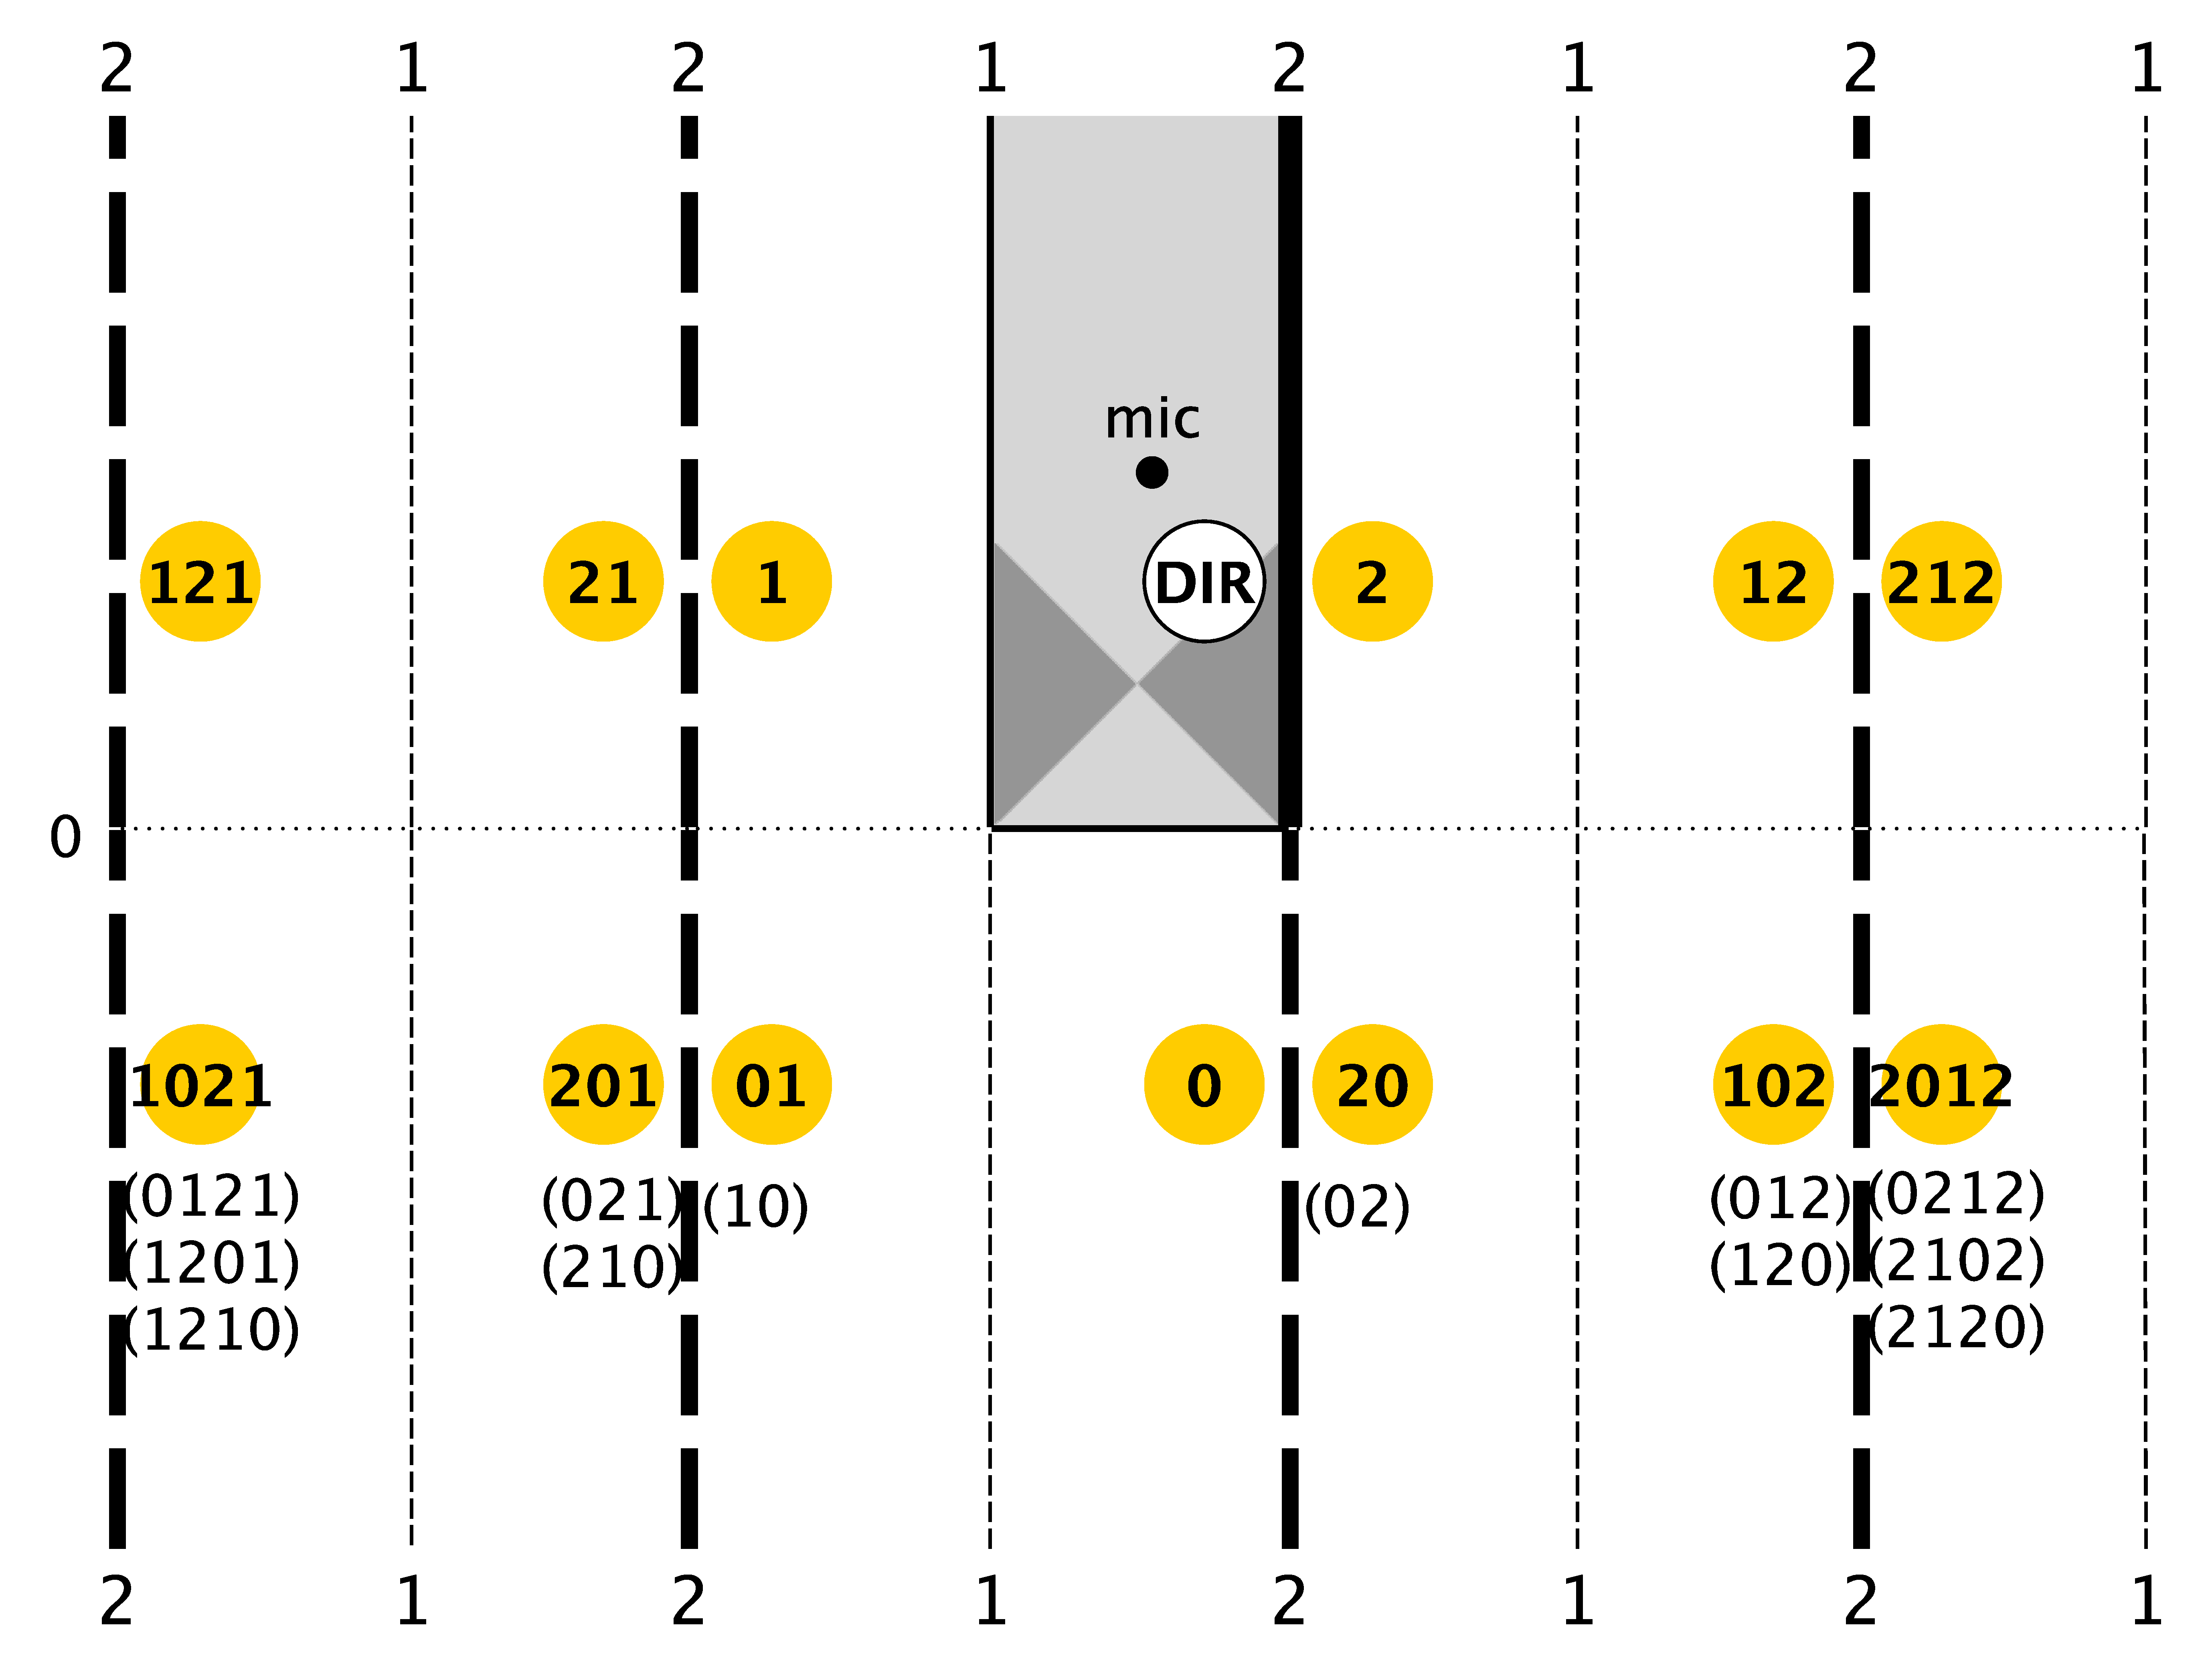
\includegraphics[width=\linewidth]{images/ISM_uncanted_v2.pdf} 
\caption{The image source model for an alley with perfectly orthogonal walls, describing the behavior of frequencies with wavelengths shorter than twice the width of the alley. Invisible sources are listed in parentheses below visible ones.} 
\end{figure}

This idealized image source model produces the impulse shown in Figure 8, specified by 480 orders of reflection, with the source and microphone in the same positions as in Fig.~2 and the dimensions of Printer's Ink Alley. The frequency response of painted concrete block was assumed independent of frequency, and a small amount of attenuation was applied to each wall reflection.

\begin{figure}[h!] \centering \includegraphics[width=\linewidth]{images/IM_480c00_irsg_cropped.pdf} \caption{Synthesized impulse response and spectrogram of the simple image model for 480 orders of reflection.} \end{figure}

In this response, we see the same diagonals of spectral zeros as in the onset in Fig.~6. %These are explained by the relationship between pairs of virtual sources located at $(x,y)$ and $(x,-y)$, and their distance to the microphone: as order increases, the difference between these two distances approaches 0. 
To explain this, we considered the microphone antennae pattern, speaker radiation pattern (facing the
west wall), and speed of sound in air, and relate visible peaks in
the measured impulse response to virtual sources in our model as in Fig.~10.

\begin{figure}[h!] \centering 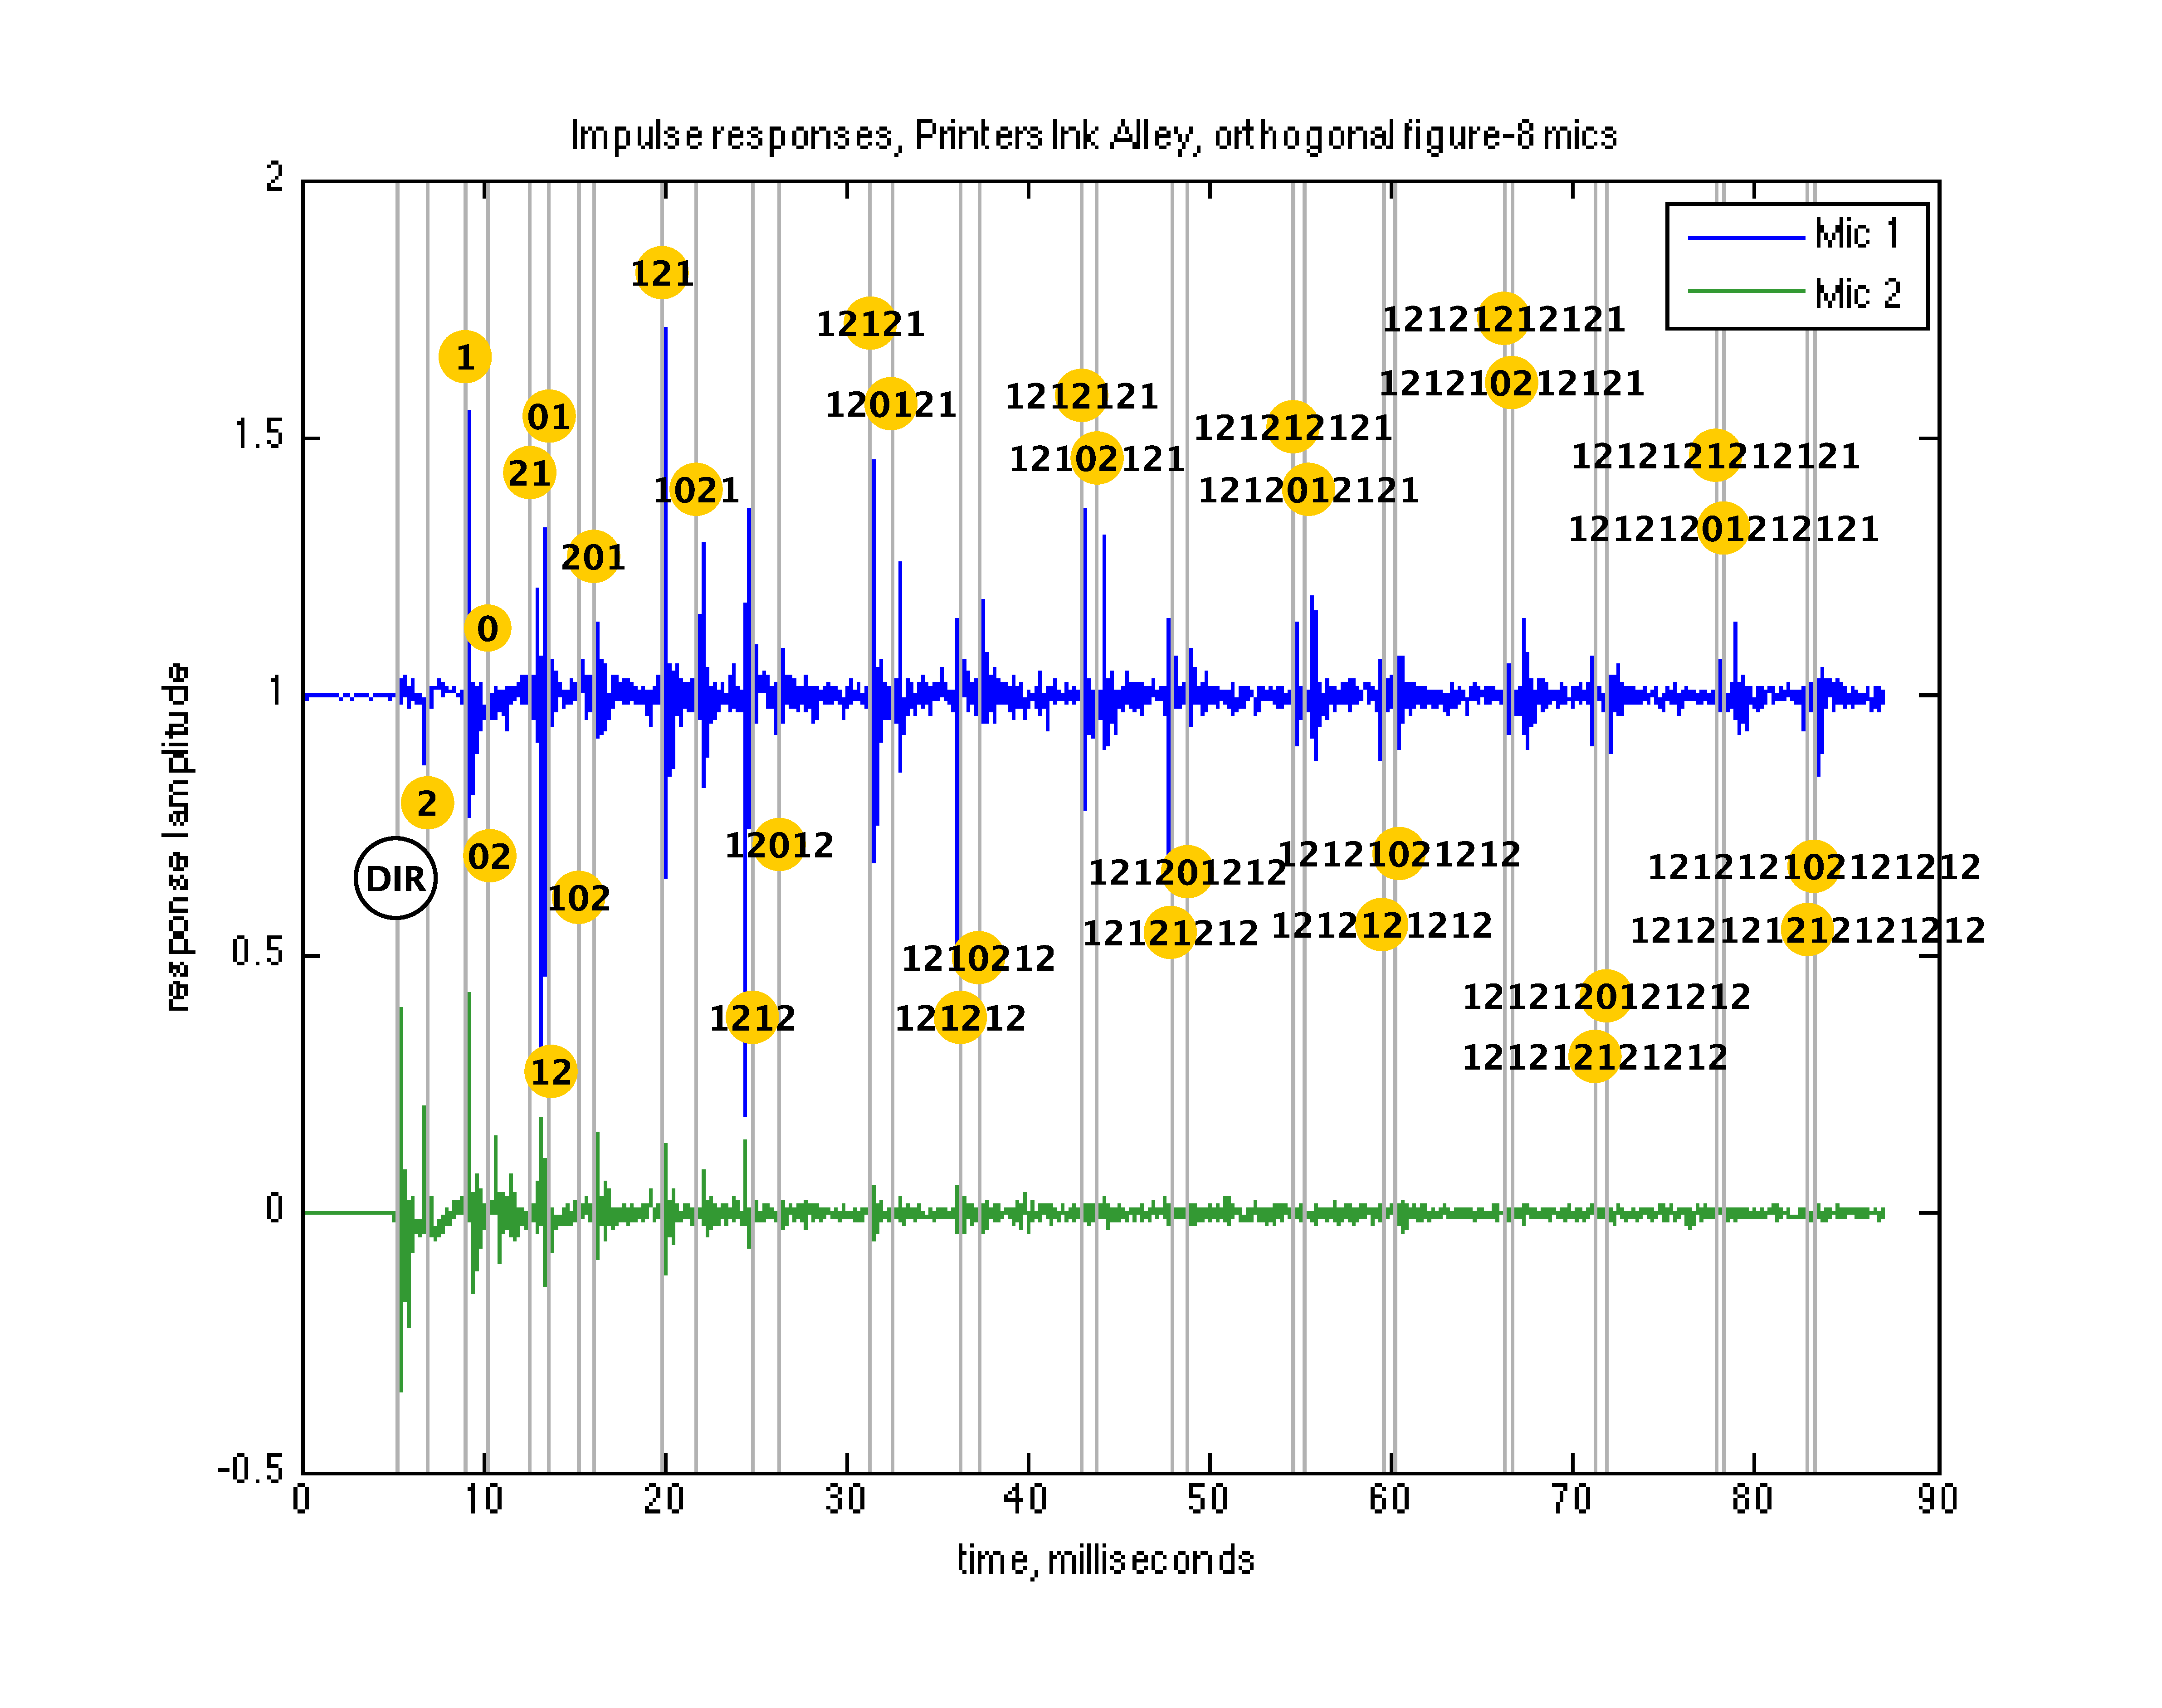
\includegraphics[width=\linewidth]{images/annotated_reflections_v2.pdf} 
\caption{Impulse response for the setup shown in Fig.~2 with speaker
  oriented to the west, first microphone channel oriented west-east, and second microphone channel oriented north-south, annotated with the virtual sources from our
  model. Because the microphones are figure-8, arrivals from the west wall (wall 1) are positive
and the east wall (wall 2) are negative. Gray, vertical lines mark the expected time of arrival of
  reflections coming from virtual sources, and the yellow circles
  label the virtual source index.} %After about 20ms, the sources
%  originating from behind the speaker (e.g., reflecting off of Wall 2)
%  are less evident, and are not labeled. The direct path, first reflection off of Wall 2,
%  and earliest reflections off of the floor are also small in Mic 1,
%  as these arrived in the null of the antennae pattern.}
\end{figure}

\begin{figure}[h!] \centering 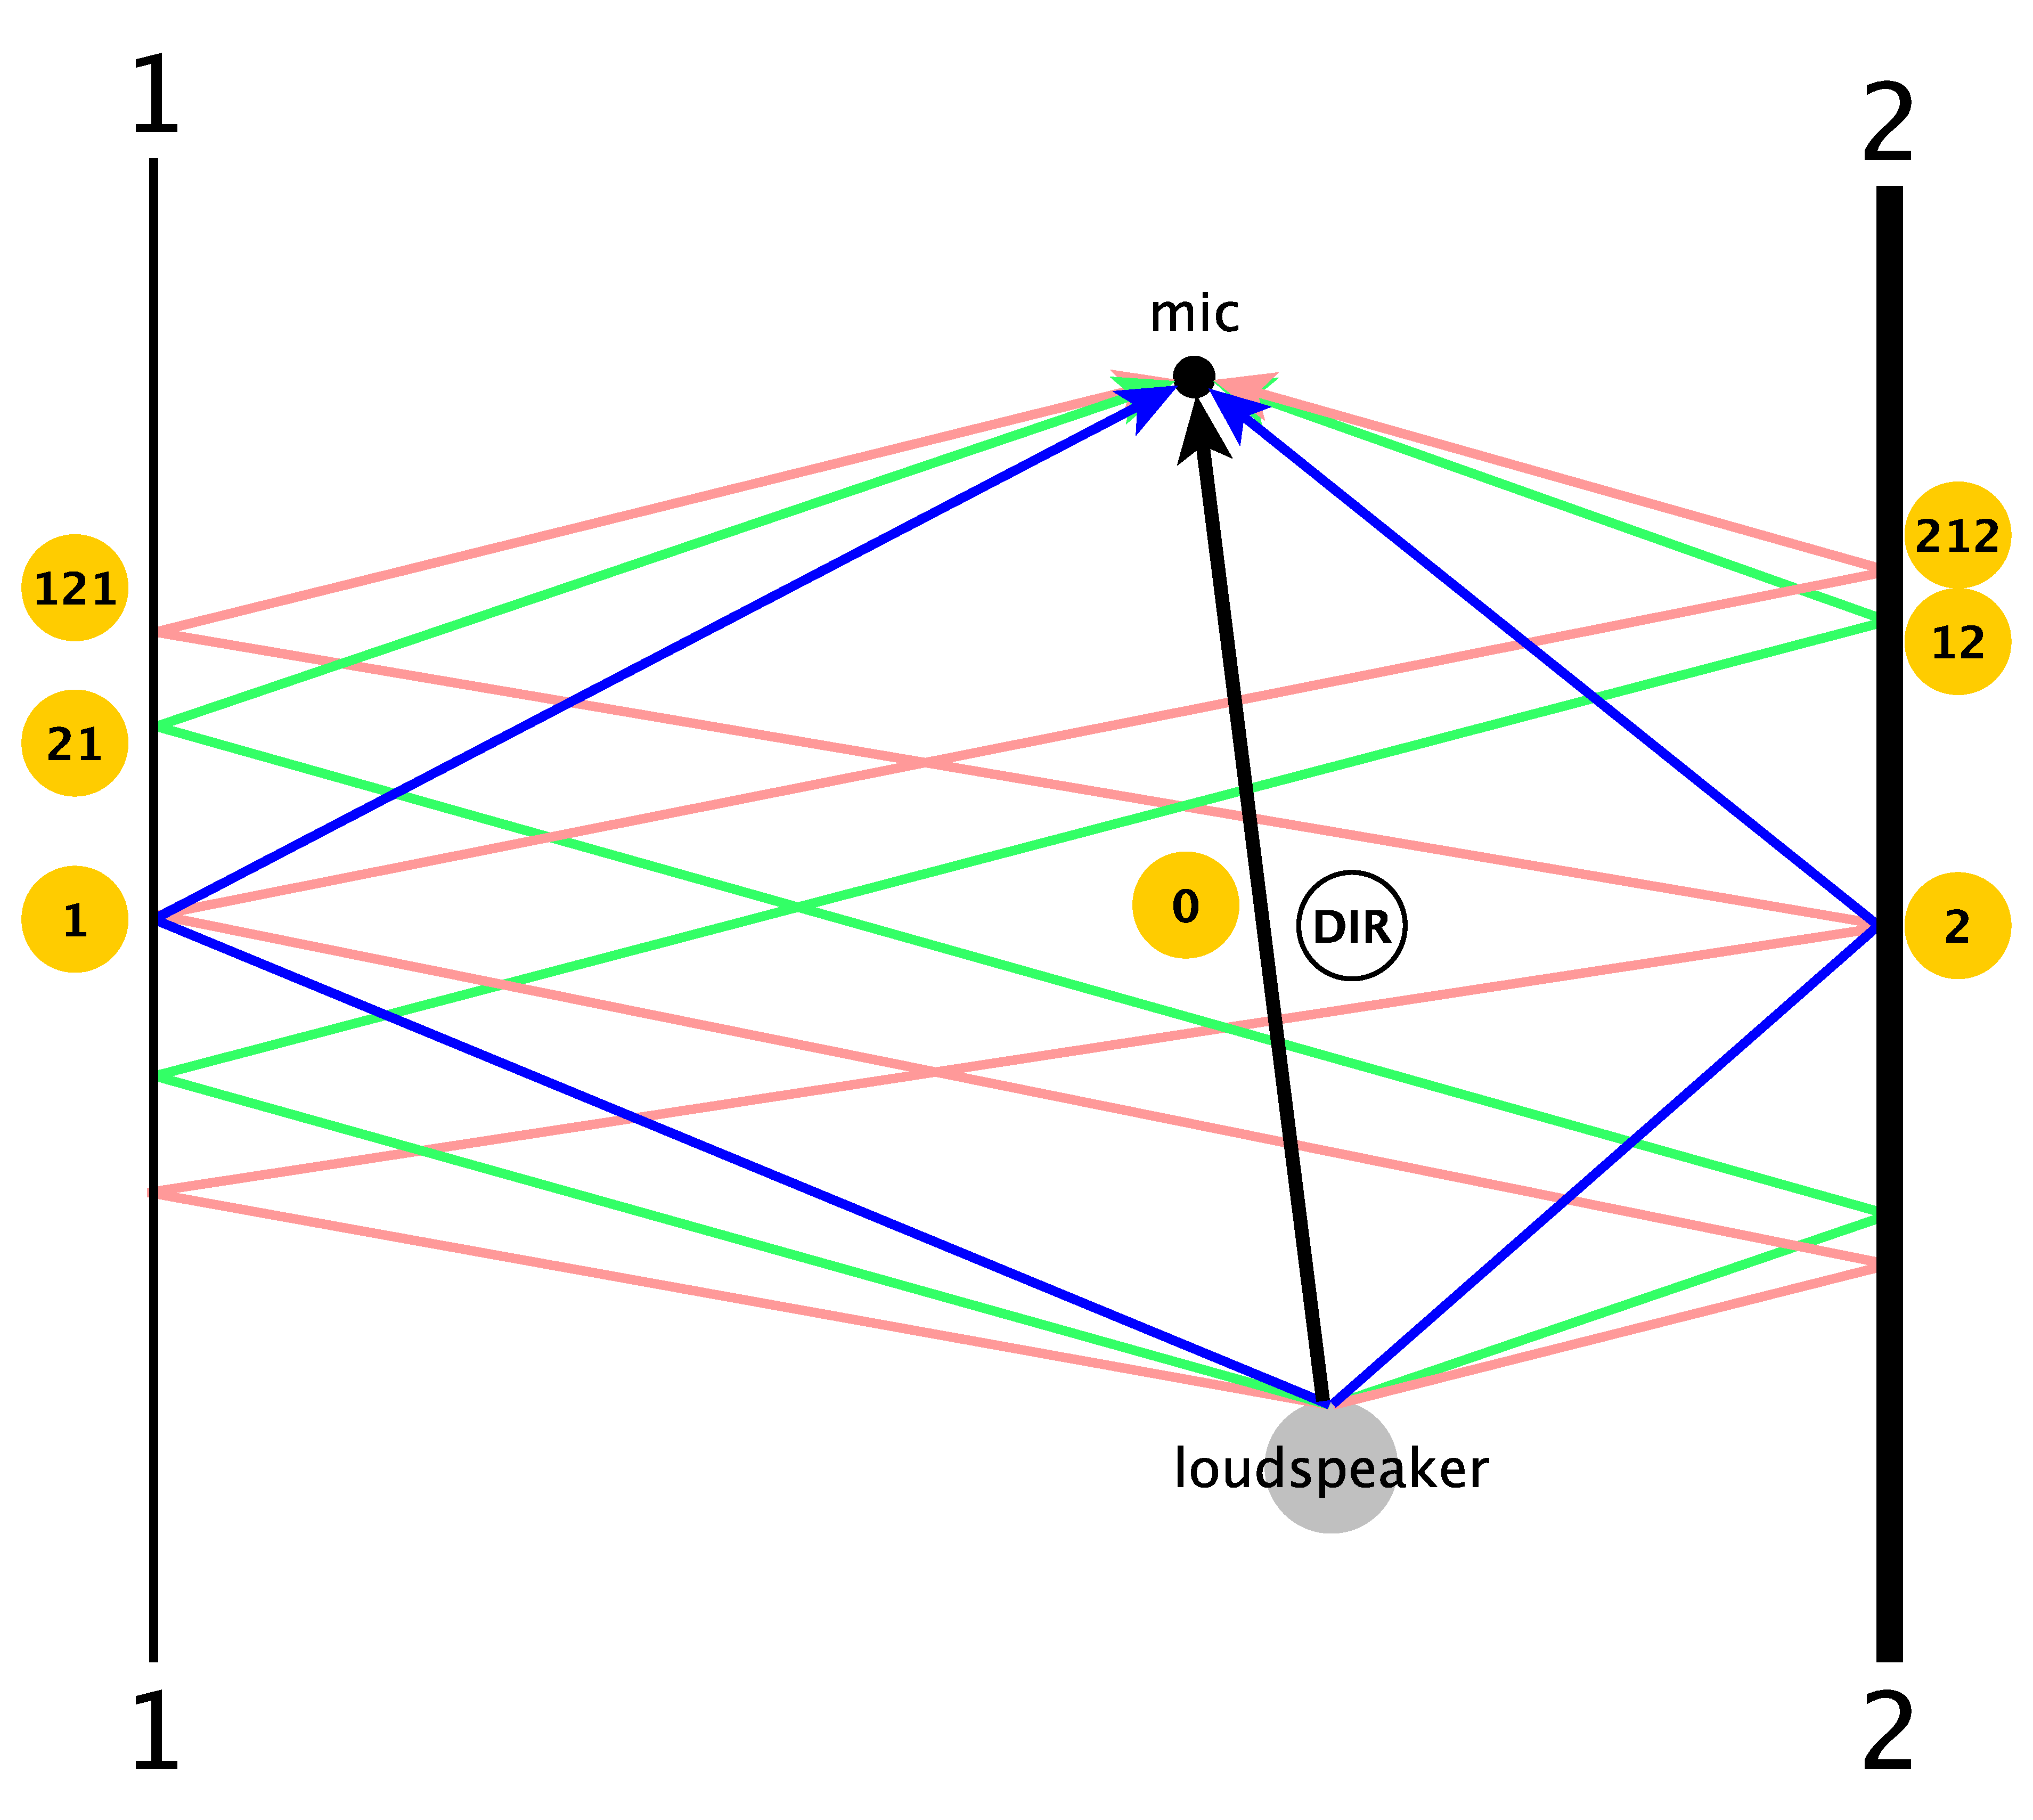
\includegraphics[width=0.7\linewidth]{images/planview_paths_v2.pdf} 
\caption{The first three orders of reflections as viewed from above the alley.} 
\end{figure}

Following the source labeled `201' in Fig.~10, no more sources beginning with `2' (to mean that they originated from the back of the speaker) are labeled, as they are buried in the noise. Hence, the sources of interest mostly originate from the front of the speaker. The very first early reflections as well as the direct path hit microphone 1 near its null, so these events are more evident in the second channel. Soon after these, a clear pattern emerges between the polarity of pulses and the source location: Sources with virtual location $(x,y)$ and $(x,-y)$ are seen in pairs in the impulse response, getting closer to one another over time as the angle between the microphone and the pair of sources approaches 0. This simple model closely describes what we see in the onset of the impulse response. 

%\begin{figure} 
%\begin{minipage}[b]{0.45\linewidth} \centering
%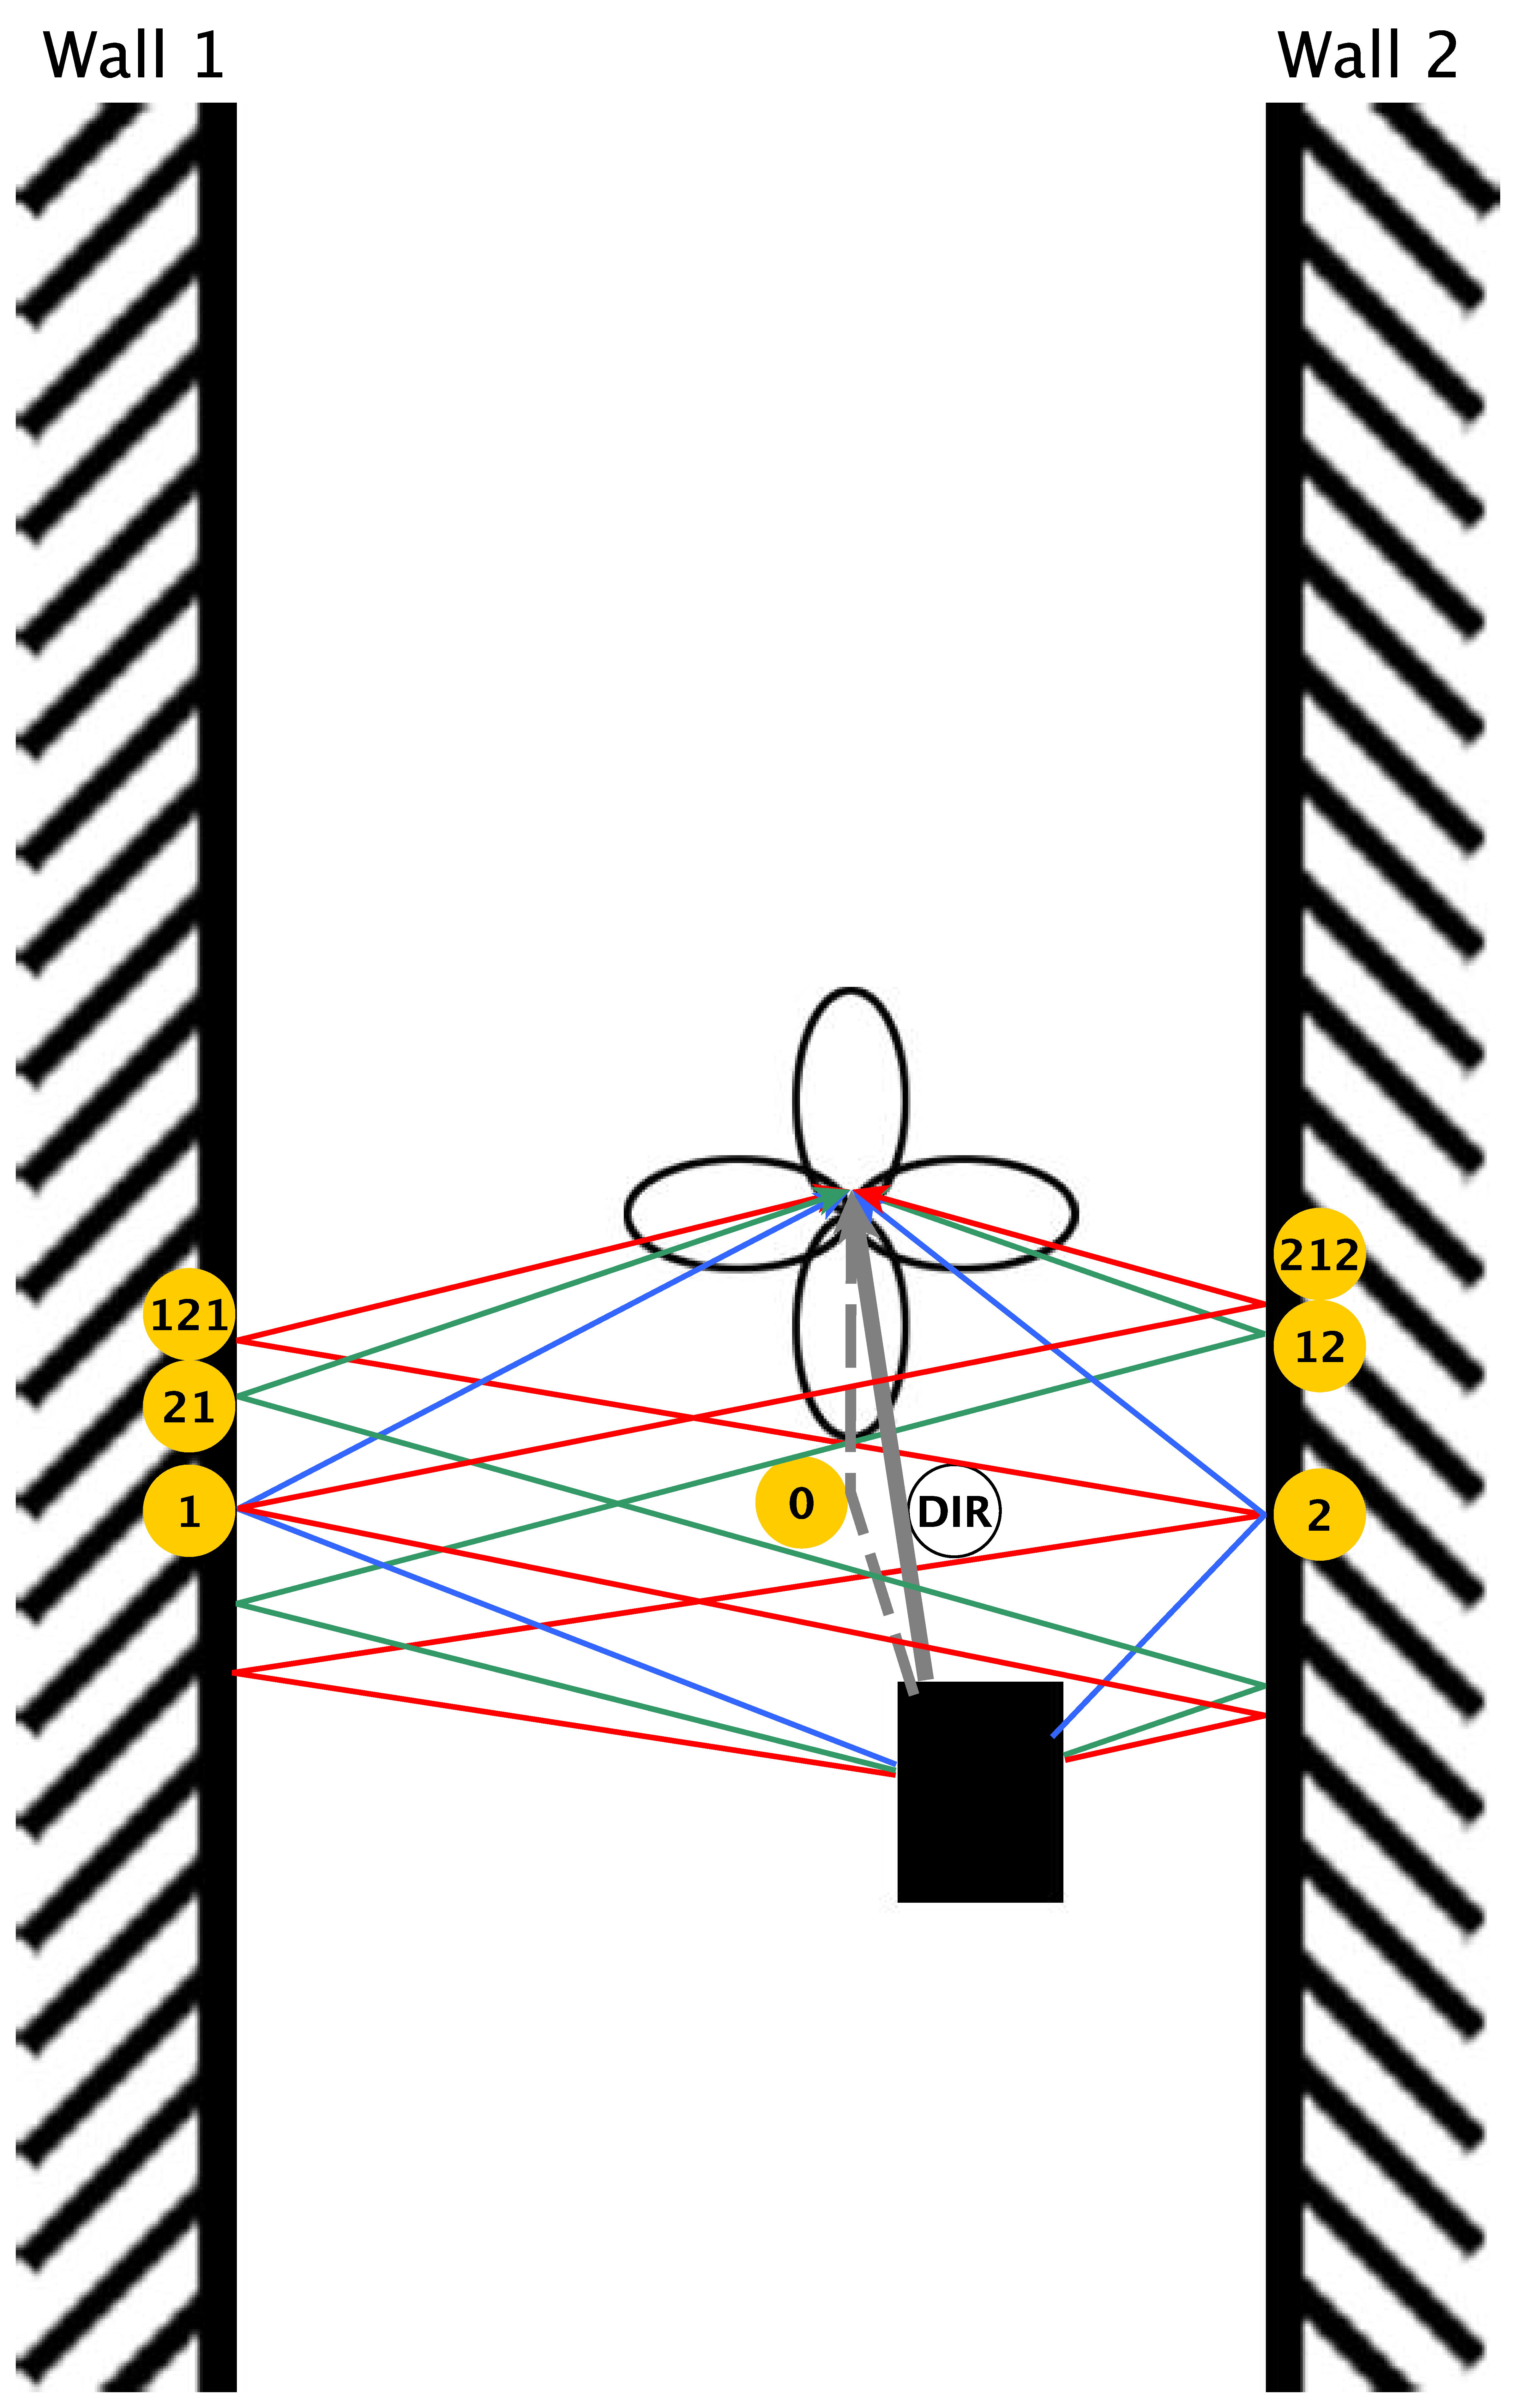
\includegraphics[width=\textwidth]{images/planview_paths.pdf}
%\end{minipage}
%\hspace{0.1\linewidth}
%\begin{minipage}[b]{0.43\linewidth} \centering
%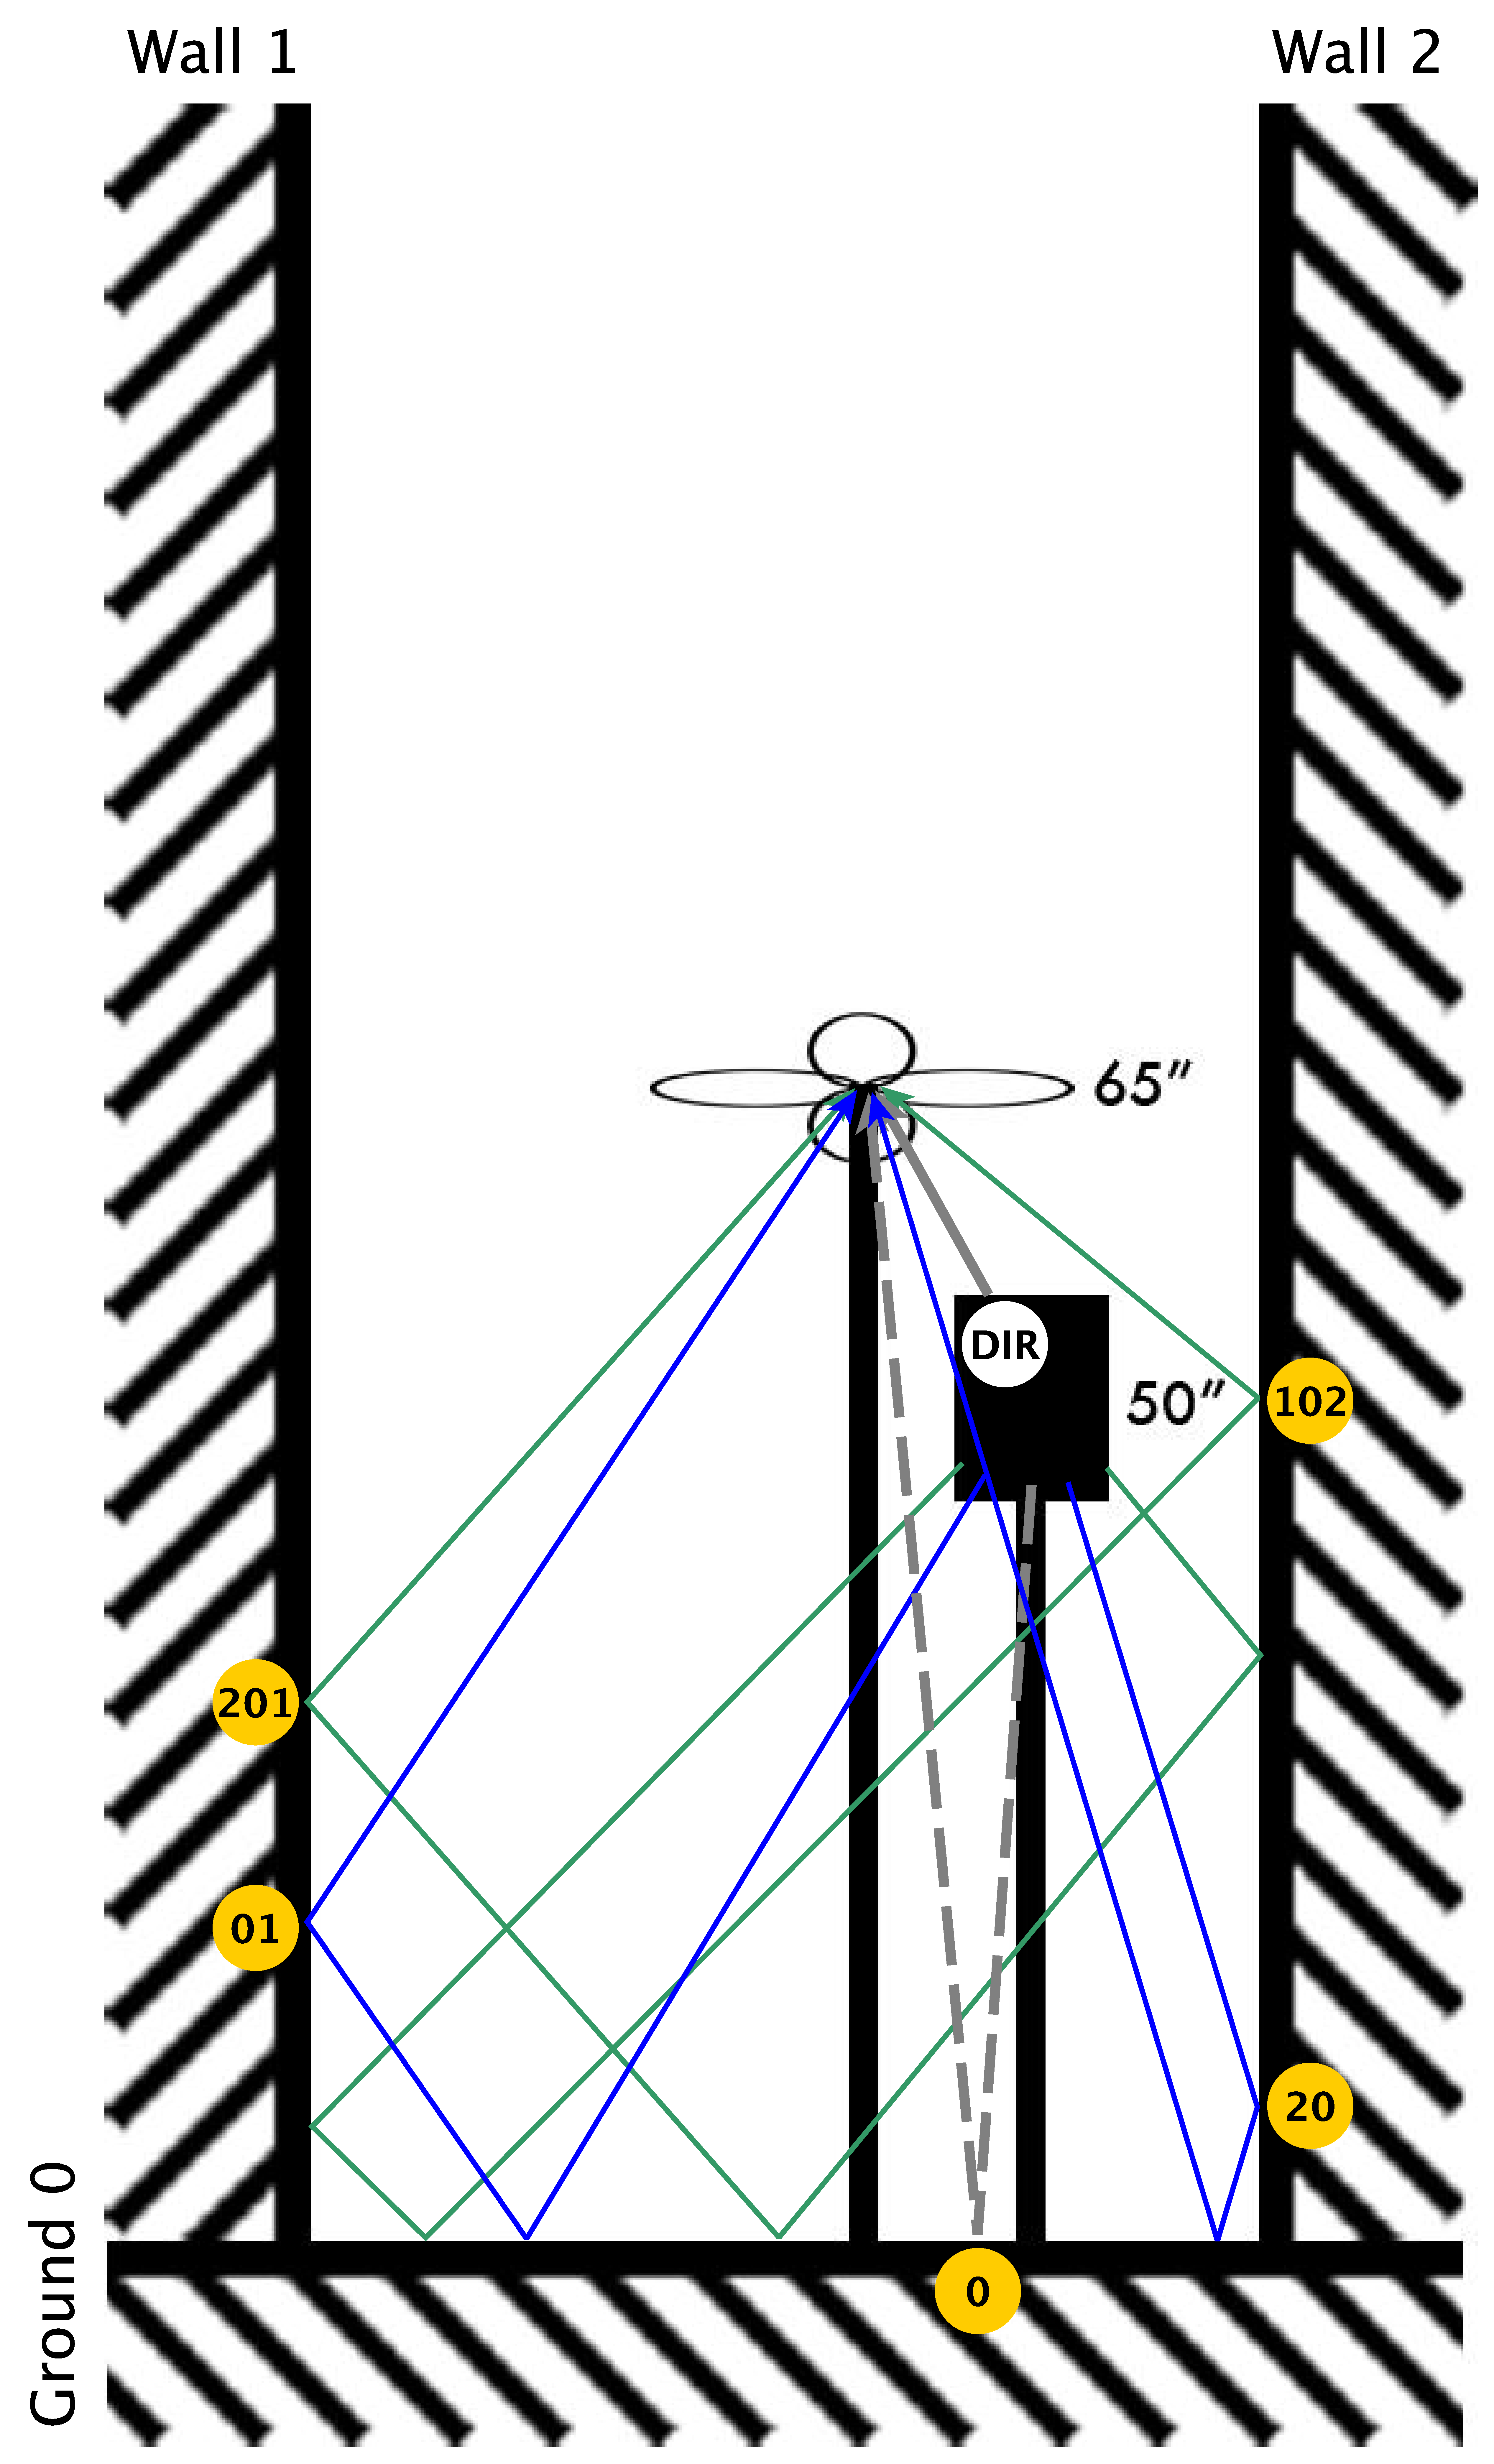
\includegraphics[width=\textwidth]{images/elevationview_paths.pdf}
%\end{minipage}
%
%\caption{Plan view (left) of our setup in ``Printer's Ink Alleyway"
%   with speaker and pair of figure-8 microphones, and elevation view of
%   the alley (right). Measurements were made with speaker oriented to
%   the north, east, and west.}
%\end{figure}


Left to explain, then, is the mode splitting we experience, and the long duration of the transient response. To resolve this, we returned to the alleyways and measured just how flat and orthogonal the walls actually were. As described in Table 1, we discovered small angles of canting in half of the walls, as well as a dip centered on the ground in Mac's Smoke Shop Alley. The resultant model, first with a 0.05m amount of canting in both walls, then with the same canting and a 0.02m dip in the center of the floor, is plotted in Figures 13--14, with the simple image model plotted in Figure 12 for comparison.

\begin{figure}[h!] \centering \includegraphics[width=\linewidth, trim=13mm 2mm 10mm 3mm, clip]{images/ISM_0m_cant_0m_dip.png} 
\caption{Virtual source locations for an alleyway with no canting. Note that invisible sources appear in the same locations as visible ones: for example, `02' and `20' are in the same location, but because the microphone is above the source, it ``sees" `20' and not the other. This illustrates the \textit{degeneracy} of sources in the simple model, which will not occur in models with canting.} 
\end{figure}

\begin{figure}[h!] \centering \includegraphics[width=\linewidth, trim=13mm 2mm 10mm 3mm, clip]{images/ISM_0pt05m_cant_0m_dip.png} 
\caption{Virtual source locations for an alleyway with both walls canted in 0.05m. The more complex geometry heeds more sources with distinct positions.} 
\end{figure}

\begin{figure}[h!] \centering \includegraphics[width=\linewidth, trim=13mm 2mm 10mm 3mm, clip]{images/ISM_0pt05m_cant_0pt02m_dip.png} 
\caption{Virtual source locations for an alleyway with both walls canted in 0.05m and a dip in the center of the ground of 0.02m. Here we see a larger vertical spread of the sources, and a higher proportion of visible sources to invisible ones.} 
\end{figure}

These more complex geometries lead to a model with sources lying on a
circle centered where the two walls would meet in space were they
sufficiently extended (the upper blue arc of sources). These are then reflected through the floor to generate another circle of sources (the lowest red arc), and finally, dense arcs of sources that intersect
both of these circles at 90 degree angles.

As the reflection order increases, the distance from the listener to the virtual sources increases roughly linearly, as does the number of distinct virtual sources that contribute to the response. Because those distinct sources arrive at distinct, irregularly spaced times (where we once had single images), the response amplitude does not decay at the $1/r$ rate of spherical spreading, but instead like $1/\sqrt{r}$ amplitude decay. %This spread in the positions of the 
These ``ripples" of concentric arcs of virtual sources generate the observed mode-splitting, which takes on the form of strong amplitude modulation due to beating frequencies.


%\begin{figure}[h!] \centering 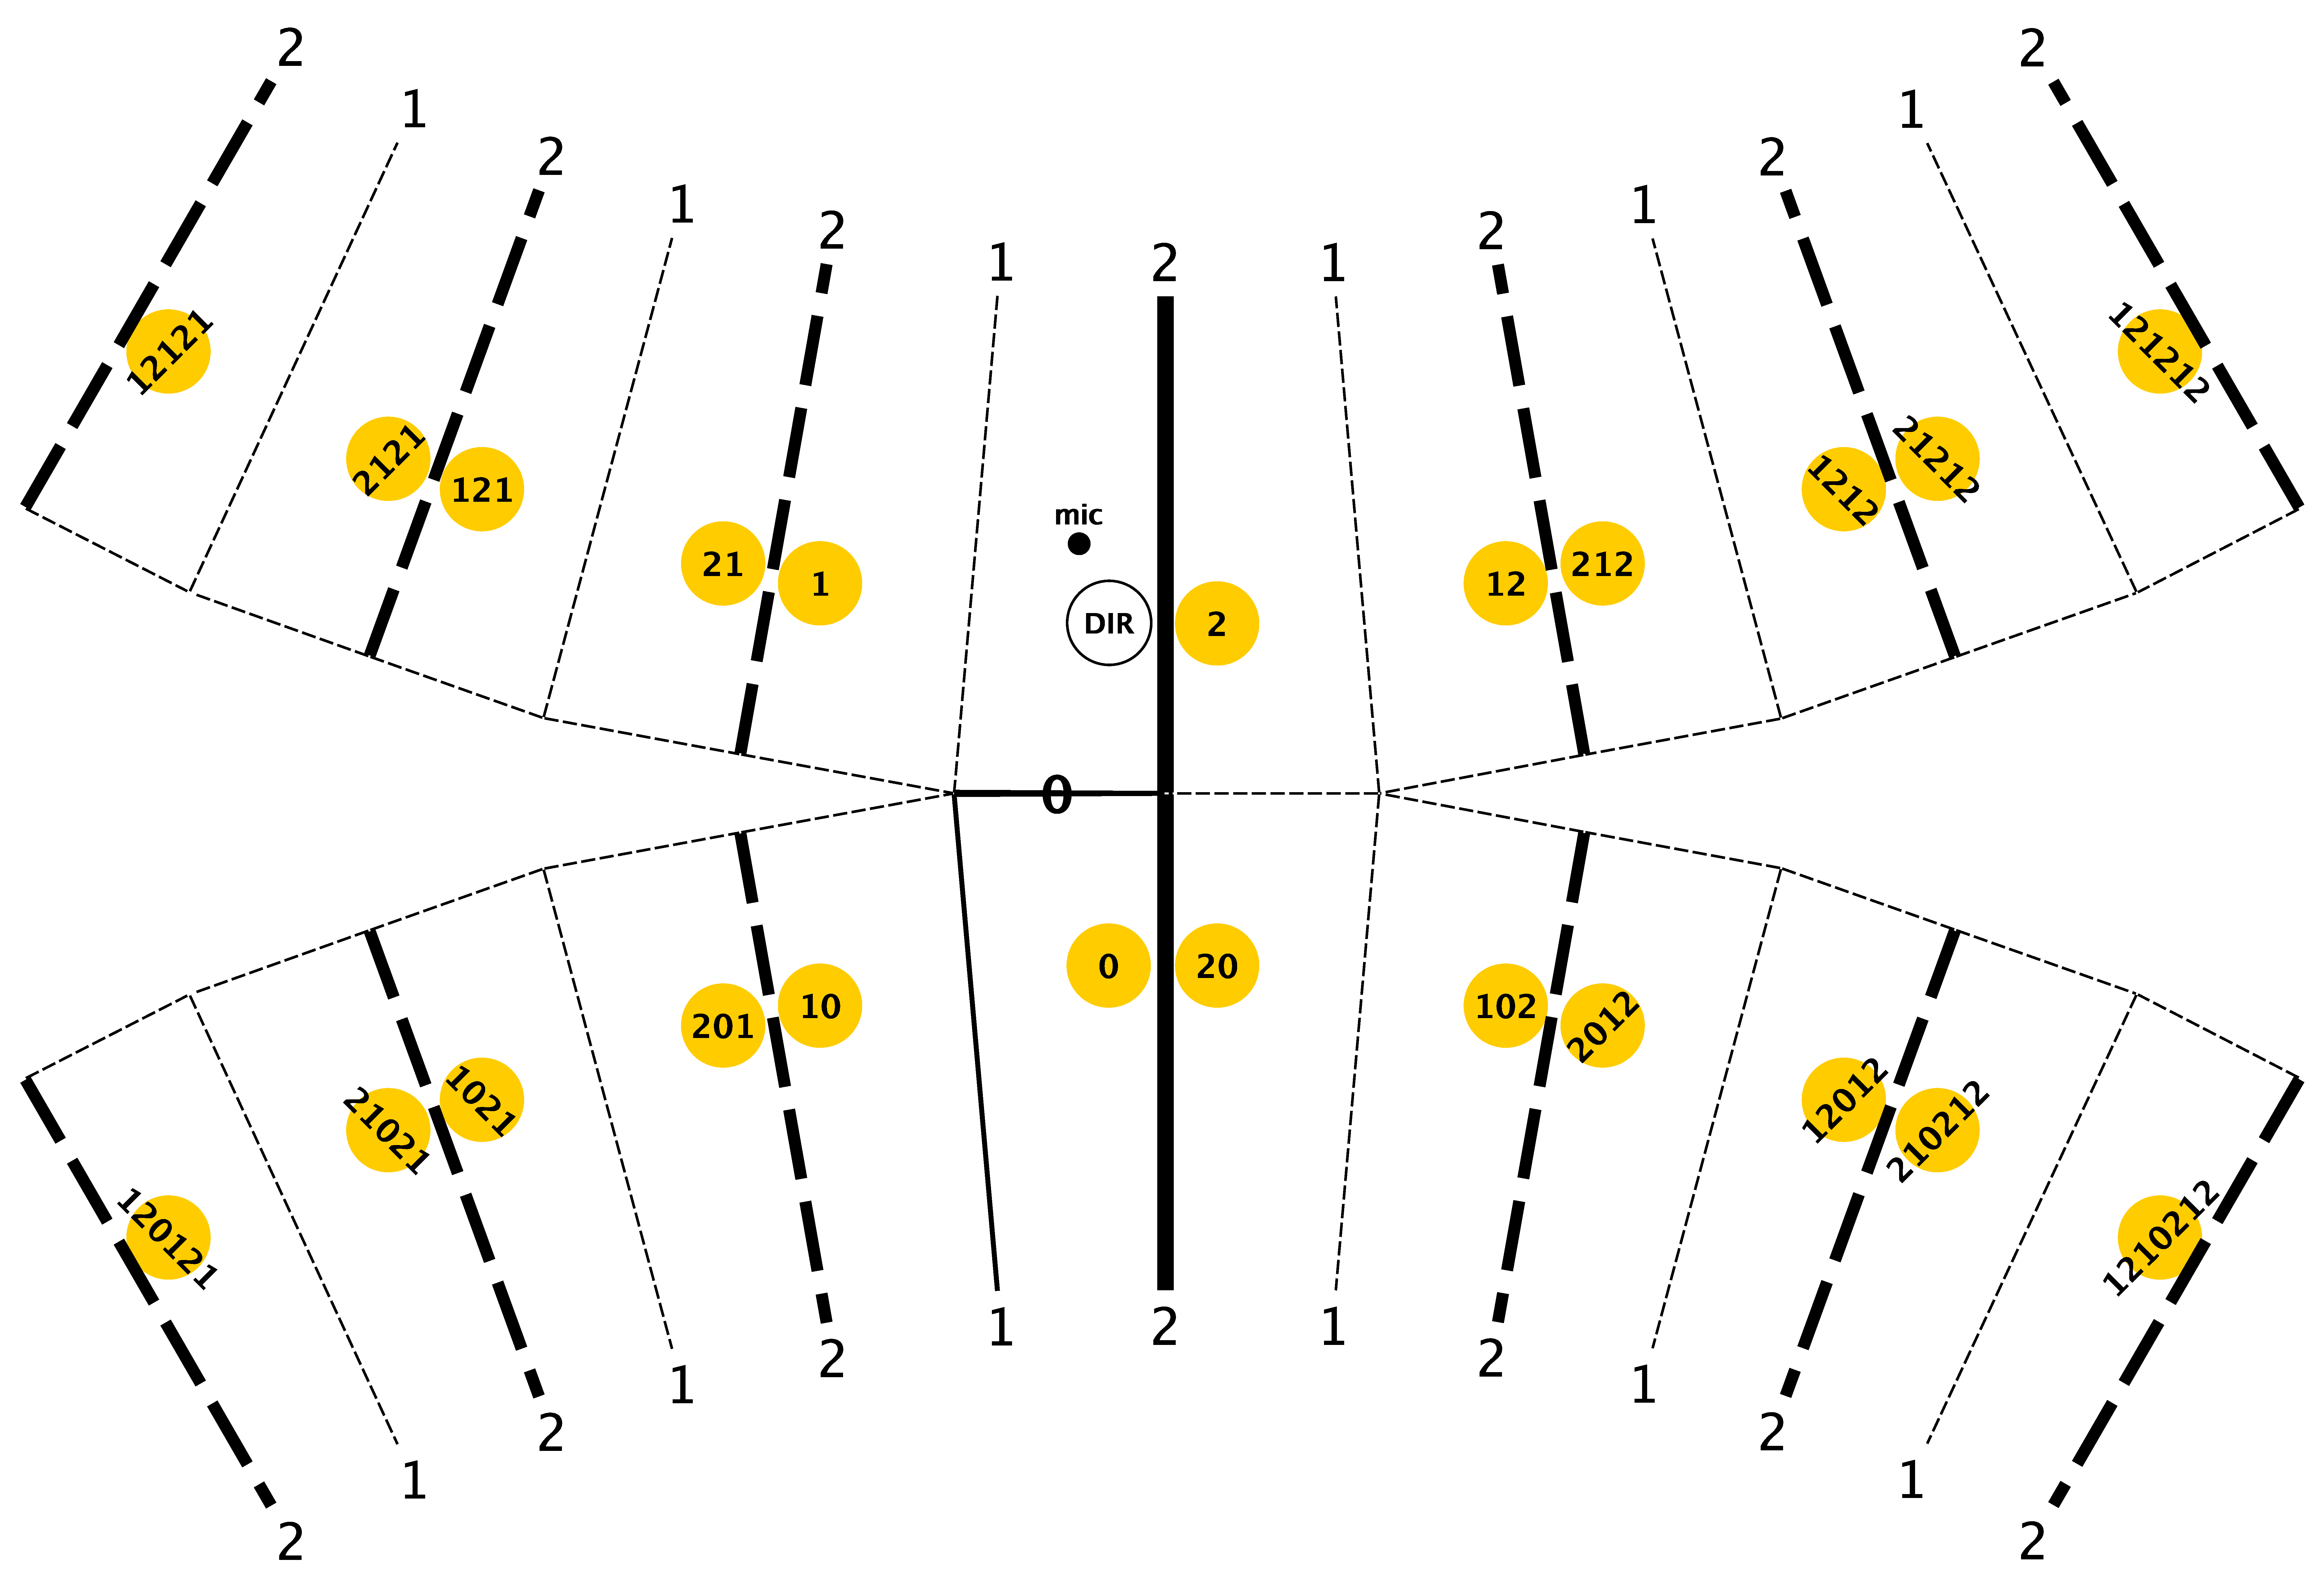
\includegraphics[width=\linewidth]{images/ISM_canted_v2.pdf} 
%\caption{The image sources lie on a circle centered at the point of the wall intersection, if they were extended infinitely through space.} 
%\end{figure}



%These ``ripples" of concentric arcs generate the amplitude modulation
%that we experience. The degree to which energy is reflected back into
%the alleyway at its upper boundary is frequency dependent, and this
%makes for frequency dependent modulation of a given mode.

%Reflection filters for the walls consisting of painted concrete block
%are virtually flat, but were accounted for according to the following
%table.
%
%\begin{table}
%\begin{center} \small
%\begin{tabular}{|l|c|c|c|c|c|c|}
%\hline
%$f$ (Hz) & 125 & 250 & 500 & 1000 & 2000 & 4000 \\
%\hline
%Gain & 0.9 & 0.95 & 0.94 & 0.93 & 0.91 & 0.92 \\
%\hline
%\end{tabular}

%\caption{Absorption coefficients for painted concrete block.} 
%\end{center} \normalsize
%\end{table}

% \subsection{Source-Microphone Distance}
From measurements taken with increasing source-microphone distance, we have one more observation about the acoustic behavior of alleyways. With increase in distance, a descending chirp frequency at the alleyway response onset becomes obvious, as illustrated in Fig.~15.

\begin{figure}[h!] \centering \includegraphics[width=\linewidth]{images/P12C_irsg_cropped.pdf} \caption{Spectrograms of four hand claps in Printer's Ink Alley, source moving away each pulse, so the source-microphone distance varies from 4' to 12' to 32' to 44' (microphone near center of alley).} \end{figure}

If the source is proximal to the listener in the alley ($<3$m), the response is more closely represented by a constant loop of arriving source reflections---e.g., the simplified image source model in Fig.~8. These arrivals produce the tone and its harmonic series that we expect, with linearly increasing distance between the listener and image sources. But when the source and listener are more distant, the low-order image sources are roughly the same distance to the listener as the original source and the later arrivals become more separated in time, creating the downward chirp frequency response. This behavior is captured by the synthesized impulse response from the idealized image model, plotted in Fig.~16.

\begin{figure}[h!] \centering \includegraphics[width=\linewidth]{images/IM_480c00_sgm_cropped.pdf} \caption{High time resolution spectrograms of the synthesized impulse response.} \end{figure}

%Measurements were made using a number of source-microphone
%distances. % , including positions between and at the walls and at various heights ranging from on the ground to eye level. 

%The impulse response resulting from the image source model with no canting in the walls is shown in Fig.~13. 

\section{Summary}

%Impulse responses generated from the image sources reproduce many of
%the features of the measured alleyway responses. The harmonic series
%and the spectral zeros rising in frequency over time are clearly
%visible, and appear to be due to the changing listener arrival times
%of signals from the image source row above the ground, relative to the
%arrival times from the image source row below the ground.
%
%
%% Where the image model fails is in the behavior of the spectral zeros
%
%The long lasting modulated tone is not present in the simple image
%source model. While the open alleyway top would create an inverting
%reflection, thus keeping energy in the alleyway, it would do so only
%at frequencies much lower than that of the frequency of the long
%lasting tone, which in our measurements is twice that of the inverse
%wall spacing. If the alleyway walls are slightly canted inward, the
%long lasting tone and its modulation can be produced. In this case,
%the modulation can be thought of as a result of the time taken for
%sound waves to reflect many times off the alleyway walls, be directed
%downwards by the wall cant, and then reflect back upwards from the
%ground.


Alleyway acoustics were explored though acoustic measurement and image method analysis. Transient response measurements using loudspeaker, hand clap, orchestral whip, and balloon pop sources reveal a series of modulated tones at frequencies consistent with the alleyway wall spacing. The impulse response onset is well-explained by an image method model of an idealized alleyway, with walls at right angles to the ground. This model produces two sets of image sources parallel to the ground and extending away from the walls. 

Differences in source-signal arrival times between the two rows are more pronounced at the beginning of the transient response than at the end, and produce a series of spectral zeros that increase in frequency with time during the impulse response onset. These zeros are also present in the measured response spectrograms, consistent with the idea that the response onset of an alleyway is well-characterized by an idealized image model.

This set of spectral zeros did not explain all of the modulation observed in the alleyway modes. By modifying the image method model to include a small amount of canting of the walls, the modes were split, consistent with the observed modulation patterns. Furthermore, the mode splitting resulted in an increasing number of visible echoes with time. This increase resulted in an atypically slow amplitude envelope decay, roughly proportional to the inverse square root of time. 

Finally, it was shown that the image source geometry was such that distant sources produce downward-going chirps at their impulse response onsets. 

% Work remains to be done in formalizing the nature of the mode splitting and the expected rate of modulation for a given tone. 

\section{Acknowledgement}
The authors would like to thank David Kerr and Sahar Tai-Seale for help with the measurements and documenting the measurement process. This research was also enabled in part by the Stanford Presidential Fund for Innovation in the Humanities, granted for ``Icons of Sound: Architectural Psychoacoustics in Byzantium," and the Stanford Arts Institute (formerly Stanford Institute for Creativity and the Arts, SiCa), {\tt http://iconsofsound.stanford.edu}.

%\begin{table*}
%\begin{center}
%\begin{tabular}{|c|l|r|}
%\hline
%234093241&23402312&3432829807434\\
%2398234&423403290&123144298\\
%2340243012597398&1245987533&24982499\\
%\hline
%\end{tabular}
%\caption{This is a two-column table.}
%\end{center}
%\end{table*}
%
%
%\begin{figure*}[tb!]
%\begin{center}
%\fbox{\vrule width0pt height 1in\vrule width6in height 0in}
%\end{center}
%\caption[2]{It is best to place to place two-column figures at the bottom
%or top of a page.}
%\end{figure*}

\bibliographystyle{IEEEtran}
% I like this better, actually: \bibliographystyle{alpha}
\bibliography{aa} % Alleyway Acoustics bibtex input file

%% \begin{thebibliography}{99}
%% \bibitem{Borish}
%% Borish, J. ``Extension of the image model to arbitrary polyhedra." J. Acoust. Soc. Am. 75, 1827 (1984).
%% \bibitem{Morse}
%% Morse, P. and K. Ingard. \emph{Theoretical Acoustics}. Princeton, NJ: Princeton University Press, 1987, pp.~471, 503, 571.
%% \end{thebibliography}

%\bibitem{DEK2}
%D. E. Knuth, {\it Selected papers on analysis of algorithms}, CSLI
%Publ., Stanford, CA, 2000; CNO
%CMP 1 762 319 
%
%\bibitem{DEK3}
%D. E. Knuth, Algorithmica {\bf 22} (1998), no.~4, 561--568; MR
%2000j:68037 
%
%\bibitem{DEK4}
%R. L. Graham, D. E. Knuth and O. Patashnik, {\it Concrete mathematics}
%(Polish), Translated from the
%second English (1994) edition by P. Chrzastowski, A. Czumaj,
%L. Gasieniec and M. Raczunas, Second
%edition, Wydawnictwo Naukowe PWN, Warsaw, 1998; MR 99m:68002


\end{document}
